\documentclass[reprint,amsmath,amssymb,aps]{revtex4-2}

\usepackage{graphicx} % Include figure files
\usepackage{dcolumn} % Align table columns on decimal point
\usepackage{bm} % bold math
\usepackage{hyperref} % add hypertext capabilities
\usepackage[spanish,mexico]{babel}
\usepackage{float} %usar [H]
\usepackage{diagbox}
\usepackage{algorithmicx}
\usepackage{algpseudocode}
\graphicspath{{imagenes/}} %Carpetas donde estaran las imagenes

\begin{document}

\preprint{APS/123-QED}

\title{Template-based Routing Generator}
\author{José de Jesús de la Rosa de la Rosa}
\email{a228835@alumnos.uaslp.mx}
\affiliation{Facultad de Ciencias, Universidad Autónoma de San Luis Potosí.}
\date{22 de junio de 2022}

\begin{abstract}
En este trabajo se presenta un generador de enrutamiento basado en plantillas (TbRG) para la automatización del diseño de circuitos integrados (IC) en tecnología CMOS (\textit{Complementary Metal-Oxide-Semiconductor}). Estos generadores utilizan plantillas que representan el diseño gráfico del circuito y enrutar circuitos, realizar cambios en el diseño de manera eficiente o migrar diseños heredados a otros nodos de tecnología. Se emplean algoritmos de búsqueda de caminos (\textit{Path-finding}), como el algoritmo de Dijkstra y el algoritmo A*, para encontrar la ruta más corta entre los puntos de origen y destino en el diseño del circuito. Se utiliza un grafo de cuadrícula para representar las capas de metal del IC, donde cada vértice representa un punto de enrutamiento y se considera una función heurística para mejorar el rendimiento del algoritmo A*. Este enfoque ofrece soluciones automáticas y eficientes para el enrutamiento de circuitos integrados, teniendo en cuenta restricciones geométricas y de rendimiento.
\end{abstract}

%\keywords{HOLA,JH,OK}

\maketitle 

\section{Introducción}

Durante años se han propuesto en la literatura técnicas de enrutamiento para la automatización del diseño de circuitos integrados digitales y analógicos. En ellas, ya se ha cubierto un amplio conjunto de restricciones geométricas para la mejora de calidad del enrutamiento, y también se han incluido progresivamente criterios relacionados con el rendimiento. Sin embargo, a medida que el diseño de circuitos mas complejos y de características particulares, como los circuitos integrados analógicos y de radiofrecuencia (A/RF)~\cite{unutulmaz, martins}, avanzan hacia nuevos nodos tecnológicos, el creciente número de reglas y restricciones de diseño, la resistencia de cables, la congestión y el crecimiento de circuitos parasíticos entre cables, impulsan constantemente las técnicas de enrutamiento automático existentes y mantienen la presión sobre su mejora. Afortunadamente, los recientes avances en las capacidades de las estaciones de trabajo modernas permitieron el crecimiento de sofisticados procesos de enrutamiento, incluidos algunos asistidos por los últimos métodos de aprendizaje automático y profundo, que ofrecen soluciones sin precedentes para la automatización de esta tarea. Sin embargo, la correlación entre las estructuras parasíticas inducidas por el enrutamiento y el comportamiento funcional del circuito dista mucho de ser sencilla, también se han propuesto técnicas de síntesis computacionalmente intensivas con inclusión de parásitos y conscientes del diseño, en las que las técnicas de enrutamiento automático desempeñan un papel decisivo.\\

\section{Path-finding algorithm}

Una de las principales técnicas es el uso de generadores de enrutamiento basados en plantillas (TbRG, \textit{Template-based routing generators}). La plantilla actúa como una representación del diseño gráfico de la tecnología, generada por el conjunto y características de los dispositivos del circuito. Son especialmente útiles cuando se debe migrar un diseño validado previamente diseñado, es decir, un diseño heredado (\textit{legacy}), a otros nodos de tecnología cercanos o se necesitan cambios en el diseño. Esta plantilla puede ser implementada como un grafo de pesos unitarios, convexo y no dirigido, donde se seleccionan un vértice origin y destino, y a través de diferentes algoritmos, encontrar el camino mas corto.

%Existe una variante del algoritmo de Dijkstra, llamado algoritmo A*, el cual tiene como objetivo únicamente el camino más corto desde una fuente específica hasta un objetivo específico, y no el árbol de caminos más corto desde una fuente específica hasta todos los objetivos posibles. Para esto es es necesario el uso de una función heurística. Para el algoritmo de Dijkstra, dado que se genera todo el árbol de la ruta más corta, cada nodo es un objetivo y no puede haber una heurística dirigida a un objetivo específico, obteniendo peor rendimiento que el algoritmo A* cuando la búsqueda del camino mas corto es solo entre dos nodos.

%\begin{figure}[H]
% 	\centering
% 	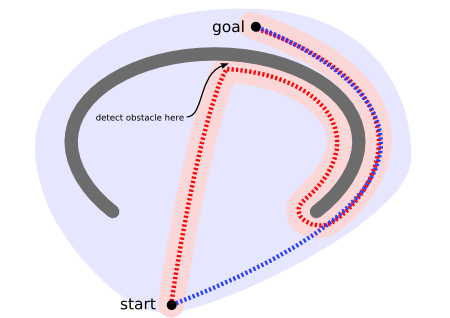
\includegraphics[width=0.48\textwidth]{concave1.png}
% 	\caption{Algoritmo pathfinding.}
% 	\label{concave1}
%\end{figure}
% 
%\begin{figure}[H]
% 	\centering
% 	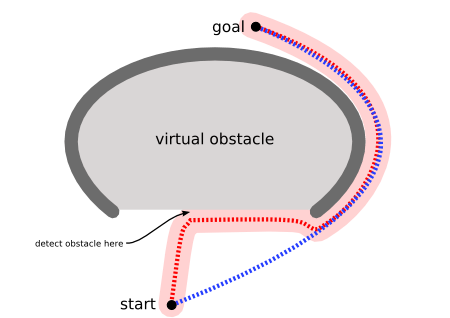
\includegraphics[width=0.48\textwidth]{concave2.png}
% 	\caption{Algoritmo pathfinding.}
% 	\label{concave2}
%\end{figure}

El algoritmo de Dijkstra, también llamado algoritmo de caminos mínimos, es un algoritmo para la determinación del camino más corto entre un vértice origen, hacia el resto de los vértices en un grafo que tiene pesos positivos en cada arista. El Algoritmo de Dijkstra funciona visitando los vértices del grafo empezando por el punto inicial fijado. A continuación, examina repetidamente el vértice más cercano aún no examinado, añadiendo sus vértices al conjunto de vértices por examinar. Se expande hacia fuera desde el punto de partida hasta alcanzar la meta. Se garantiza que el Algoritmo de Dijkstra encuentra el camino más corto desde el punto de partida hasta la meta, siempre que ninguna de las aristas tenga un coste negativo. En el siguiente diagrama, el cuadrado rosa es el punto de partida, el cuadrado azul es la meta, y las áreas de color azulado muestran las áreas que el algoritmo de Dijkstra escaneó. Las zonas más claras son las más alejadas del punto de partida y, por tanto, constituyen la "frontera" de la exploración:

\begin{figure}[H]
 	\centering
 	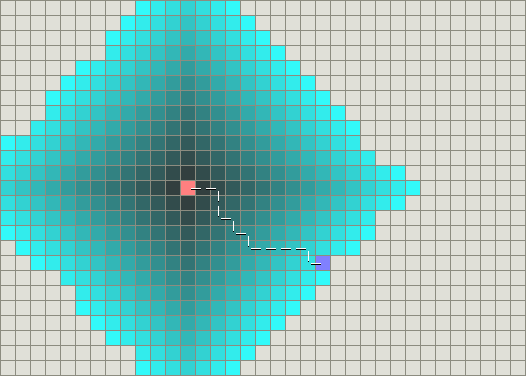
\includegraphics[width=0.48\textwidth]{dijkstra.png}
 	\caption{Demostración del algoritmo de Dijkstra en un grafo de rejilla.}
 	\label{dijkstra}
\end{figure}

El algoritmo Greedy Best-First-Search funciona de forma similar, salvo que tiene una estimación (llamada función heurística ó simplemente heurística) de la distancia a la que se encuentra un vértice de la meta. En lugar de seleccionar el vértice más cercano al punto de partida, selecciona el más cercano a la meta. No se garantiza que el algoritmo encuentre el camino más corto. Sin embargo, se ejecuta mucho más rápido que el algoritmo de Dijkstra porque utiliza la función heurística para guiar su camino hacia la meta muy rápidamente. Por ejemplo, si el objetivo está al sur de la posición inicial, el algoritmo Greedy Best-First-Search tenderá a centrarse en los caminos que conducen hacia el sur. En el siguiente diagrama, el amarillo representa los nodos con un valor heurístico alto (coste alto para llegar a la meta) y el negro los nodos con un valor heurístico bajo (coste bajo para llegar a la meta). Esto demuestra que el algoritmo Greedy Best-First-Search puede encontrar caminos muy rápidamente en comparación con el algoritmo de Dijkstra:

\begin{figure}[H]
 	\centering
 	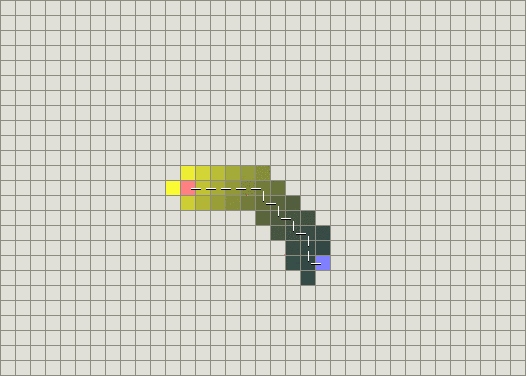
\includegraphics[width=0.48\textwidth]{greedy.png}
 	\caption{Demostración del algoritmo Greedy Best-First-Search en un grafo de rejilla.}
 	\label{a}
\end{figure}

Sin embargo, ambos ejemplos ilustran el caso más sencillo: cuando el mapa no tiene obstáculos y el camino más corto es realmente una línea recta. Consideremos el obstáculo cóncavo: el Algoritmo de Dijkstra es más difícil, pero se garantiza que encuentra el camino más corto:

\begin{figure}[H]
 	\centering
 	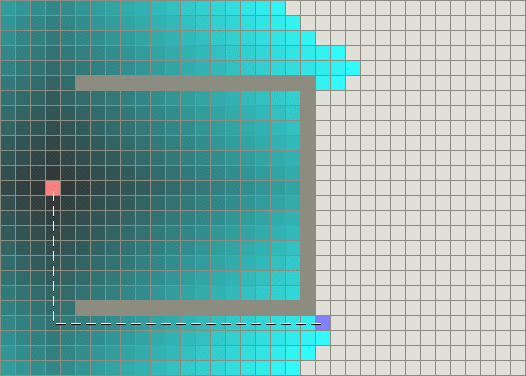
\includegraphics[width=0.48\textwidth]{dijkstra-trap.png}
 	\caption{Demostración del algoritmo de Dijkstra en un grafo de rejilla con un obstáculo cóncavo.}
 	\label{dijkstra-trap}
\end{figure}
 
Por otro lado, el algoritmo Greedy realiza menos trabajo, pero su camino no es tan bueno. El problema es que intenta avanzar hacia la meta aunque no sea el camino correcto. Como sólo tiene en cuenta el coste de llegar a la meta e ignora el coste del camino hasta ahora, sigue avanzando aunque el camino se haya hecho muy largo.
 
\begin{figure}[H]
 	\centering
 	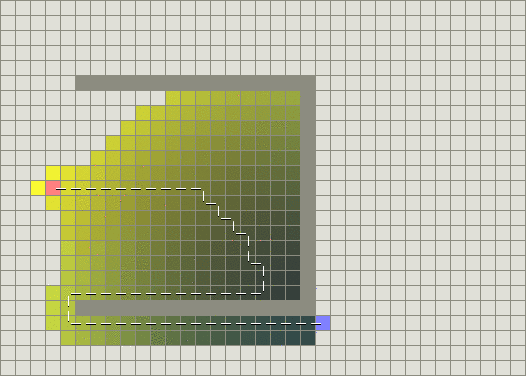
\includegraphics[width=0.48\textwidth]{greedy-trap.png}
 	\caption{Demostración del algoritmo Greedy Best-First-Search en un grafo de rejilla con un obstáculo cóncavo.}
 	\label{a-trap}
\end{figure}


El algoritmo A* (A estrella) es como el algoritmo de Dijkstra en el sentido de que puede utilizarse para encontrar el camino más corto. A* se parece al algoritmo Greedy Best-First-Search en que puede utilizar una heurística para guiarse. En el caso simple, es tan rápido como el algoritmo Greedy Best-First-Search como se muestra en la Figura~\ref{a-star}:

\begin{figure}[H]
	\centering
	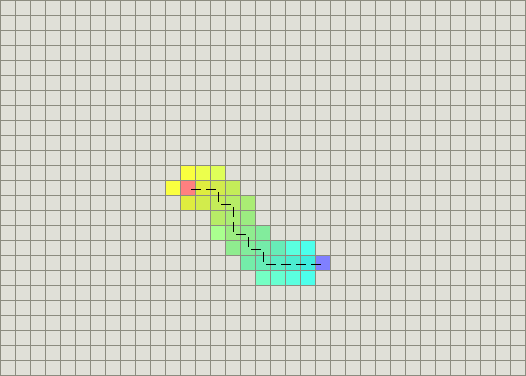
\includegraphics[width=0.48\textwidth]{a-star.png}
	\caption{Demostración del algoritmo A* en un grafo de rejilla.}
	\label{a-star}
\end{figure}

Esto se debe a que combina la información que utiliza el Algoritmo de Dijkstra (favoreciendo los vértices con menor coste desde el origen) y la información que utiliza el algoritmo Greedy Best-First-Search (favoreciendo los vértices que están cerca de la meta). En la literatura se explica que una función $g(n)$ representa el coste exacto del camino desde el punto de partida hasta cualquier vértice n, y otra función $h(n)$ representa el coste heurístico estimado desde el vértice n hasta la meta. En los diagramas anteriores, el amarillo ($h$) representa los vértices alejados de la meta y el verde azulado ($g$) representa los vértices alejados del punto de partida y en la Figura~\ref{a-star-trap} se muestra la combinación de ambos. El algoritmo A* equilibra ambos a medida que se desplaza desde el punto de partida hasta la meta. Cada vez que pasa por el bucle principal, la función $f(n)=g(n)+h(n)$ examina el vértice n que tiene el valor más bajo.

\begin{figure}[H]
	\centering
	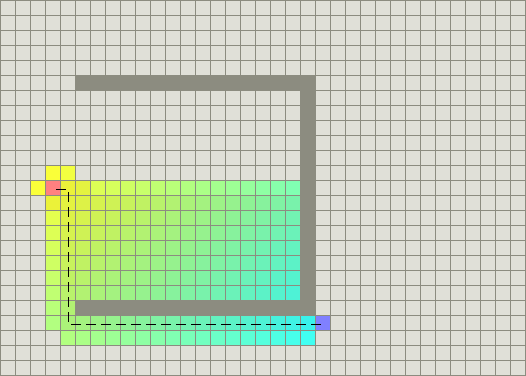
\includegraphics[width=0.48\textwidth]{a-star-trap.png}
	\caption{Demostración del algoritmo A* en un grafo de rejilla con un obstáculo cóncavo.}
	\label{a-star-trap}
\end{figure}

La heurística en una cuadrícula cuadrada donde se puede mover en 4 direcciones debe ser D (escala) veces la distancia de \textit{Manhattan}, como a continuación se describe:

\begin{algorithmic}
    \Function{Heurística}{$nodo$}
        \State $dx \gets \text{abs}(nodo.x - \text{meta.x})$
        \State $dy \gets \text{abs}(nodo.y - \text{meta.y})$
        \State \Return $D \cdot (dx + dy)$
    \EndFunction
\end{algorithmic}


La elección de D se lleva a cabo de la siguiente manera: se emplea una escala que se ajuste a la función de costes. Para los mejores caminos, y una heurística ``admisible'', se establece D al menor coste entre cuadrados adyacentes. En ausencia de obstáculos, y en un terreno que tenga el mínimo coste de movimiento D, acercarse un paso a la meta debería aumentar g en D y disminuir h en D. Cuando sumas los dos, f (que se establece en g + h) permanecerá igual; eso es señal de que la heurística y las escalas de la función de coste coinciden. También puedes renunciar a caminos óptimos para hacer que A* corra más rápido aumentando D, o disminuyendo la relación entre los costes de arista más bajos y más altos.

\section{Celdas estándar}

Para modelar los circuitos integrados como grafos, se sigue un enfoque basado en la información proporcionada por las celdas estándar de la biblioteca utilizada. Se extrae la ubicación de las distintas capas de metal, en particular, en este trabajo se consideró únicamente la primer capa de metal (M1). Con el fin de representar estas capas de metal en un grafo, se empleó un grafo de cuadrícula, donde cada vértice representa un punto a través del cual se puede enrutar un cable de metal. Se utilizan vértices ``disponibles'' y ``no disponibles'', siendo los no disponibles aquellos puntos donde ya existe metal o alguna otra obstrucción por donde no sea posible enrutar, asumiendo una separación de un micrómetro entre cada vértice en el diseño del circuito. El peso de cada arista se estableció en 1 junto con el uso de la función heurística para el algoritmo A*. En la Figura~\ref{inv} se muestra el layout de un inversor, en donde la capa de color rojo, indica la capa de metal 1, esta información es interpretada del archivo LEF de la biblioteca de celdas estándar. En la Figura~\ref{inv_m1} se muestra únicamente la capa de metal 1 y los rectángulos que conforma el inversor, de los cuales es generado el grafo cuadricular.

\begin{figure}[H]
	\centering
	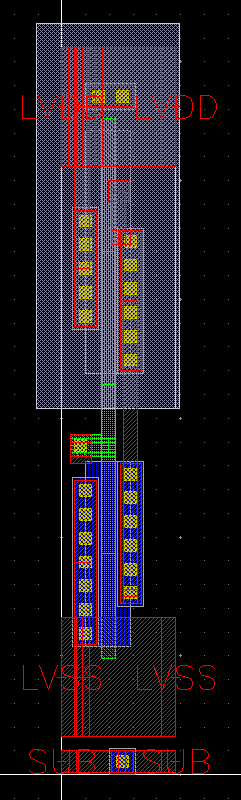
\includegraphics[scale=0.65]{inv.png}
	\caption{Layout de un inversor en tecnología CMOS.}
	\label{inv}
\end{figure}

\begin{figure}[H]
	\centering
	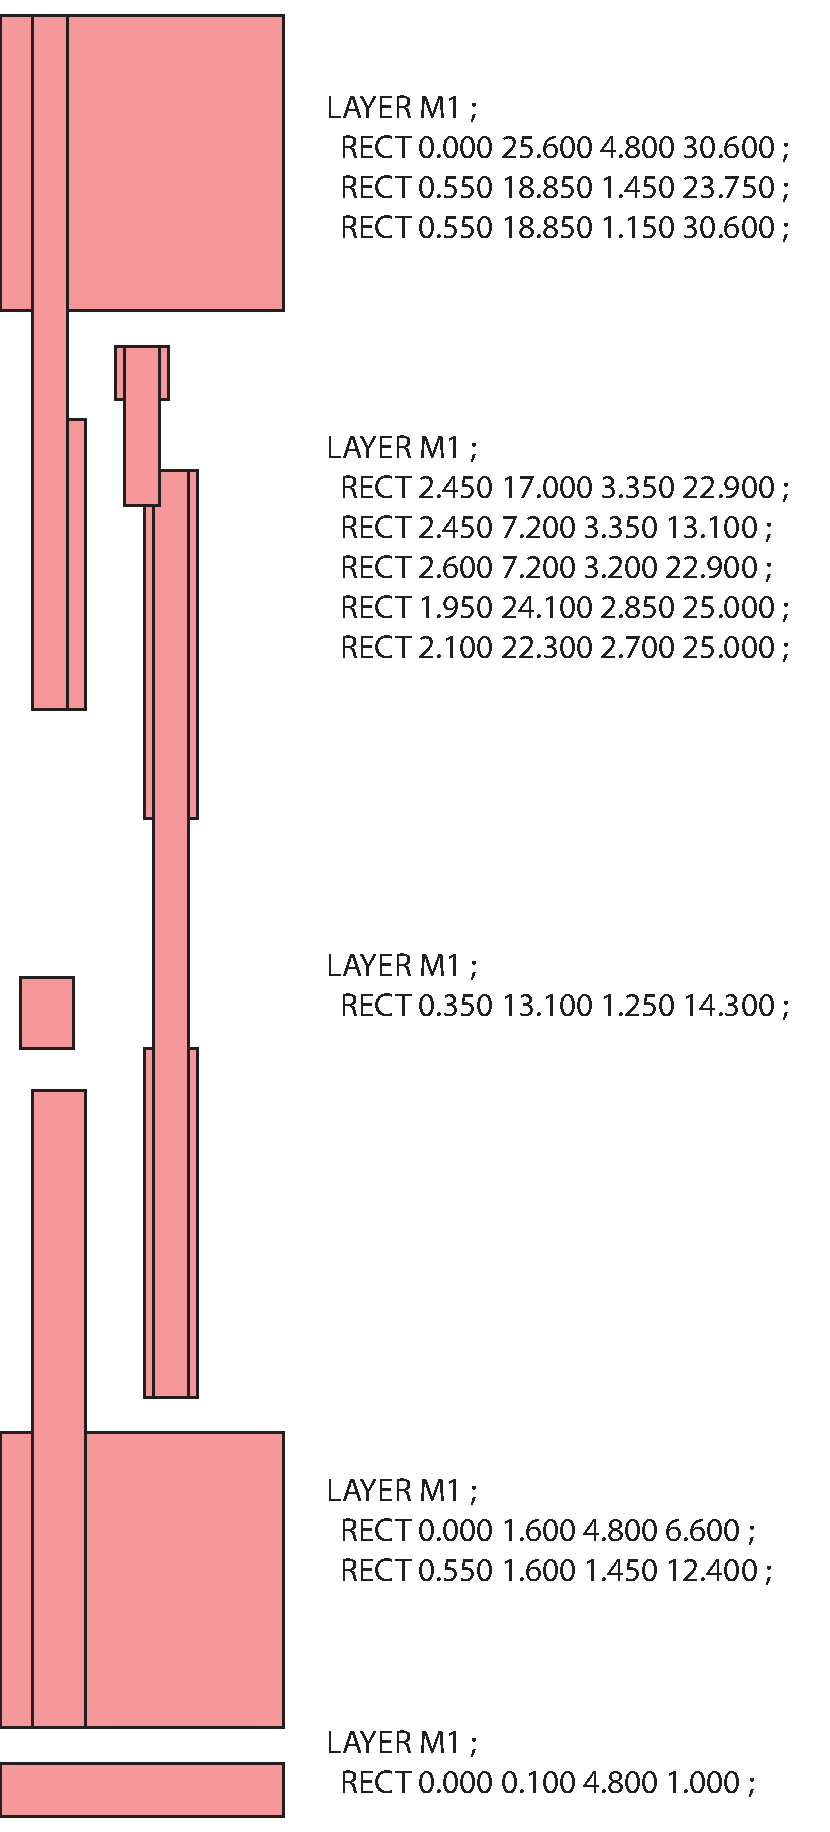
\includegraphics[width=0.29\textwidth]{inv_m1.pdf}
	\caption{Capa del primer metal de un inversor.}
	\label{inv_m1}
\end{figure}

Finalmente, con la información del grafo, se fijan los nodos de origen y destino, y se emplea el algoritmo A* para el cálculo de la ruta más corta. Para obtener más información sobre la implementación del algoritmo de enrutamiento utilizado, se puede consultar el repositorio en GitHub~\footnote{\url{https://github.com/NanophotonIICOs/router-dijkstra}}.


\section{Resultados y trabajo a futuro}

Con la información de la grid almacenada en un archivo, el script del algoritmo A* genera el camino más corto. Además, haciendo uso de la librería libbmp, se generan imágenes de la grid que resaltan visualmente dicho camino, como se muestra en la Figura~\ref{cuadricula_final2}. Estas imágenes proporcionan una representación visual del resultado obtenido por el algoritmo, permitiendo una mejor comprensión de la ruta óptima seleccionada dentro de la grid. La librería libbmp facilita la creación de estas imágenes al proporcionar funcionalidades específicas para el manejo y la manipulación de archivos de imagen en formato BMP.

\begin{figure}[H]
	\centering
	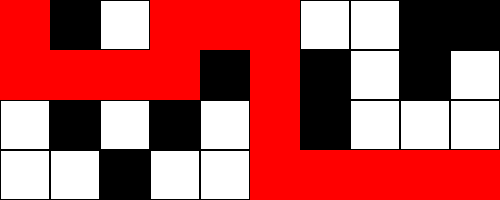
\includegraphics[width=0.4\textwidth]{cuadricula_final2.png}
	\caption{Diagrama de un grafo de rejilla con el camino mas corto del vértice en la esquina superior izquierda al vértice inferior derecho.}
	\label{cuadricula_final2}
\end{figure}

Un potencial problema que surge al generar el enrutamiento en circuitos de gran tamaño, es la cantidad de vértices de la grid generada, debido a la granularidad de 1 micrómetro entre cada vértice del grafo, como se muestra en la Figura~\ref{cuadricula_final}. La manipulación de esta cantidad masiva de información puede resultar en una implementación inviable en términos de tiempo y recursos computacionales. Por lo tanto, se continúa trabajando en el desarrollo de representaciones alternativas de los circuitos integrados, como el uso de grafos Hanan. Esta representación ofrece una manera más eficiente de modelar y abordar el enrutamiento en circuitos de mayor escala, al reducir la complejidad del grafo y permitir una mejor gestión de los recursos disponibles. La cuadrícula de Hanan de un conjunto finito S de puntos en el plano se obtiene construyendo líneas verticales y horizontales que conectan cada punto en S, formando un grafo con una menor cantidad de vértices en comparación con la implementación actual. Esta reducción en la cantidad de vértices facilita la tarea de enrutamiento y optimiza el uso de recursos, brindando una solución más eficiente para la representación de circuitos integrados de mayor escala.

\begin{figure}[H]
	\centering
	\includegraphics[width=0.5\textwidth]{cuadricula_final.png}
	\caption{Diagrama de un grafo de rejilla de gran escala con el camino mas corto del vértice en la esquina superior izquierda al vértice inferior derecho.}
	\label{cuadricula_final}
\end{figure}

En adición, se continúa trabajando en el proceso de place \& route a partir de una descripción de alto nivel, con el objetivo de que la herramienta sea capaz de tomar esta representación y generar el layout final del circuito integrado. El enfoque de place \& route busca optimizar la ubicación de las celdas en el chip y determinar las rutas de conexión más eficientes entre ellas. Mediante el uso de algoritmos y técnicas avanzadas, se pretende automatizar este proceso y mejorar la productividad en el diseño de circuitos integrados, reduciendo los tiempos de desarrollo y maximizando el rendimiento y eficiencia del diseño resultante. Esta integración entre la representación de alto nivel y el proceso de place \& route representa un paso importante hacia la generación automática y rápida de los layouts finales de los circuitos integrados.

\section{Conclusiones}
conclusiones
  
\bibliographystyle{unsrtnat}
\nocite{*}
\bibliography{citas}% Produces the bibliography via BibTeX.

\end{document}
